%
% $RCSfile: analysis.tex,v $
%
% Copyright (C) 2002-2008. Christian Heller.
%
% Permission is granted to copy, distribute and/or modify this document
% under the terms of the GNU Free Documentation License, Version 1.1 or
% any later version published by the Free Software Foundation; with no
% Invariant Sections, with no Front-Cover Texts and with no Back-Cover
% Texts. A copy of the license is included in the section entitled
% "GNU Free Documentation License".
%
% http://www.cybop.net
% - Cybernetics Oriented Programming -
%
% http://www.resmedicinae.org
% - Information in Medicine -
%
% Version: $Revision: 1.1 $ $Date: 2008-08-19 20:41:05 $ $Author: christian $
% Authors: Christian Heller <christian.heller@tuxtax.de>
%

\section{Analysis}
\label{analysis_heading}
\index{Res Medicinae Requirements Analysis}
\index{Software Engineering Process}
\index{SEP}
\index{Electronic Health Record}
\index{EHR}

Abiding by the standard \emph{Software Engineering Process} (SEP) (chapter
\ref{software_engineering_process_heading}), a \emph{Requirements Analysis}
stood as first activity for the development of \emph{Res Medicinae}. The
following sections will give a brief overview of some requirements and current
modelling trends, concerning the \emph{Electronic Health Record} (EHR). They do
\emph{not} try to replace more comprehensive works written on the subject.

%
% $RCSfile: requirements_document.tex,v $
%
% Copyright (C) 2002-2008. Christian Heller.
%
% Permission is granted to copy, distribute and/or modify this document
% under the terms of the GNU Free Documentation License, Version 1.1 or
% any later version published by the Free Software Foundation; with no
% Invariant Sections, with no Front-Cover Texts and with no Back-Cover
% Texts. A copy of the license is included in the section entitled
% "GNU Free Documentation License".
%
% http://www.cybop.net
% - Cybernetics Oriented Programming -
%
% http://www.resmedicinae.org
% - Information in Medicine -
%
% Version: $Revision: 1.1 $ $Date: 2008-08-19 20:41:08 $ $Author: christian $
% Authors: Christian Heller <christian.heller@tuxtax.de>
%

\subsection{Requirements Document}
\label{requirements_document_heading}
\index{Res Medicinae Requirements Document}
\index{DocBook DTD}
\index{The Linux Documentation Project}
\index{TLDP}

With the help of German medical doctors, a \emph{Requirements Document}
\cite{resmedicinae2001} was created and is meanwhile being updated and extended
since about five years. It basically describes an EHR and the information it
should include.

Since the document itself is just a hierarchical model consisting of parts, it
can well be represented in CYBOL. Unfortunately, a document processor that can
read and render CYBOL, in the style of \emph{LaTeX} \cite{latex}, has not been
written to date (although CYBOI might integrate this functionality one day). It
was therefore decided to write the requirements document in SGML/ XML, using
the \emph{DocBook} DTD \cite{docbook} and tools described in
\emph{The Linux Documentation Project} (TLDP) \cite{linuxdoc}.

%
% $RCSfile: ehr_and_co.tex,v $
%
% Copyright (C) 2002-2008. Christian Heller.
%
% Permission is granted to copy, distribute and/or modify this document
% under the terms of the GNU Free Documentation License, Version 1.1 or
% any later version published by the Free Software Foundation; with no
% Invariant Sections, with no Front-Cover Texts and with no Back-Cover
% Texts. A copy of the license is included in the section entitled
% "GNU Free Documentation License".
%
% http://www.cybop.net
% - Cybernetics Oriented Programming -
%
% http://www.resmedicinae.org
% - Information in Medicine -
%
% Version: $Revision: 1.1 $ $Date: 2008-08-19 20:41:06 $ $Author: christian $
% Authors: Christian Heller <christian.heller@tuxtax.de>
%

\subsection{EHR \& Co.}
\label{ehr_and_co_heading}
\index{Electronic Health Record}
\index{EHR}
\index{Personal Health Record}
\index{PHR}
\index{Virtual Health Record}
\index{VHR}
\index{Virtual Patient Record}
\index{VPR}
\index{Electronic Medical Record}
\index{EMR}
\index{Electronic Patient Record}
\index{EPR}
\index{Computer-based Patient Record}
\index{CPR}
\index{Computerised Patient Record}
\index{CPR}
\index{Computerised Medical Record}
\index{CMR}
\index{Automated Medical Record}
\index{AMR}
\index{Digital Medical Record}
\index{DMR}
\index{Patient Carried Record}
\index{PCR}
\index{Patient Medical Record}
\index{PMR}
\index{Integrated Care Record}
\index{ICR}
\index{Electronic Medical Infrastructure}
\index{EMI}
\index{Lifetime Data Repository}
\index{LDR}

Besides the now quite common term \emph{Electronic Health Record} (EHR), some
publications, experts or companies also talk of \cite{marietti, waegemann}:

\begin{itemize}
    \item[-] \emph{Personal Health Record} (PHR)
    \item[-] \emph{Virtual Health Record} (VHR)
    \item[-] \emph{Virtual Patient Record} (VPR)
    \item[-] \emph{Electronic Medical Record} (EMR)
    \item[-] \emph{Electronic Patient Record} (EPR)
    \item[-] \emph{Computer-based Patient Record} (CPR)
    \item[-] \emph{Computerised Patient Record} (CPR)
    \item[-] \emph{Computerised Medical Record} (CMR)
    \item[-] \emph{Automated Medical Record} (AMR)
    \item[-] \emph{Digital Medical Record} (DMR)
    \item[-] \emph{Patient Carried Record} (PCR)
    \item[-] \emph{Patient Medical Record} (PMR)
    \item[-] \emph{Integrated Care Record} (ICR)
    \item[-] \emph{Electronic Medical Infrastructure} (EMI)
    \item[-] \emph{Lifetime Data Repository} (LDR)
\end{itemize}

and state differences in their contents, access, maintainer, place of storage,
technology or other aspects. David Kibbe, for example, as cited by Jennifer
Bush \cite{bush}, says:

\begin{quote}
    There's recently been a subtle shift in terminology. EMR connotes a tool
    that's for doctors only and something that replaces the paper record with a
    database. EHR connotes more of a connectivity tool that not only includes
    the patient and may even be used by the patient, but also provides a set of
    tools to improve work-flow efficiency and quality of care in doctors' offices.

    \ldots\ An EHR should include a detailed clinical documentation function;
    prescription ordering and management capabilities; a secure messaging
    system; lab and test result reporting functions; evidence-based health
    guidelines; secure patient access to health records; a public health
    reporting- and tracking system; mapping to clinical- and standard code sets
    and the ability to interface with leading practice management software.
\end{quote}

In essence, however, most of the above-listed terms are considered synonymous,
since their definitions, if existent at all, differ just in nuances. Charlene
Marietti, who investigated in this subject, writes \cite{marietti}:

\begin{quote}
    Meanwhile, most practical people don't see a big difference between the CPR
    and the EMR and the many other terms that exist.
\end{quote}

Therefore, this work further on sticks to the term \emph{EHR} and wants it
understood as general description for either of the other terms mentioned
above.

%
% $RCSfile: episode_based.tex,v $
%
% Copyright (C) 2002-2008. Christian Heller.
%
% Permission is granted to copy, distribute and/or modify this document
% under the terms of the GNU Free Documentation License, Version 1.1 or
% any later version published by the Free Software Foundation; with no
% Invariant Sections, with no Front-Cover Texts and with no Back-Cover
% Texts. A copy of the license is included in the section entitled
% "GNU Free Documentation License".
%
% http://www.cybop.net
% - Cybernetics Oriented Programming -
%
% http://www.resmedicinae.org
% - Information in Medicine -
%
% Version: $Revision: 1.1 $ $Date: 2008-08-19 20:41:06 $ $Author: christian $
% Authors: Christian Heller <christian.heller@tuxtax.de>
%

\subsection{Episode Based}
\label{episode_based_heading}
\index{Episode Based EHR}
\index{Patient Centered Medical Record}
\index{Health Issue of an Episode Based EHR}
\index{Clinical Episode of an Episode Based EHR}
\index{Clinical Encounter of an Episode Based EHR}
\index{Clinical Item of an Episode Based EHR}
\index{Partial Contact of an Episode Based EHR}
\index{Problem Oriented Medical Record}
\index{POMR}

Historically, it took a long time until the concept of a modern EHR crystalised
out. An early form of a time-oriented medical record stems from Hippocrates
(5th century BC) who wanted to accurately reflect the course of a disease and
indicate its possible causes. In 1907, the \emph{Mayo Clinic} (formed by the
American surgeon William Mayo) adopted one separate file for each patient, to
be able to obtain a better overview of his complete disease history. This
innovation was the origin of the \emph{Patient Centered Medical Record} as
known today, as \cite{mihandbook} means.

The discussion on how to model an ideal EHR already lasts for decades and has
not finished. Recent proposals brought in some new perspectives and ideas. One
of them turns around the so-called \emph{Episode-based} EHR \cite{westerhof}.
In the centre of these considerations stands a structure that is described in a
more pragmatic way by Karsten Hilbert of GNUmed \cite{gnumed}. He sees a
complex EHR as hierarchical composition of the following items:

\begin{itemize}
    \item[-] Health Issue
    \item[-] Clinical Episode
    \item[-] Clinical Encounter
    \item[-] Clinical Item
\end{itemize}

The additional concept of a \emph{Partial Contact} as known from the Dutch
\emph{Episode Model} does not integrate into this hierarchy. But after Hilbert,
\emph{Partial Contacts} could be easily derived from existing EHR data by
aggregating all \emph{Clinical Items} that belong to the same
\emph{Clinical Encounter} and the same \emph{Clinical Episode}.

\emph{Clinical Items} are typically elements in the \emph{SOAP} format of
progress notes, as known from the \emph{Problem Oriented Medical Record} (POMR)
\cite{weed} that was introduced by Lawrence L. Weed in the 1960s. SOAP stands
for:

\begin{itemize}
    \item[-] \emph{Subjective:} Complaints as phrased by the patient
    \item[-] \emph{Objective:} Findings of physicians and nurses
    \item[-] \emph{Assessment:} Test results and conclusions, such as a diagnosis
    \item[-] \emph{Plan:} Medical plan, for example treatment or policy
\end{itemize}

%
% $RCSfile: evidence_based.tex,v $
%
% Copyright (C) 2002-2008. Christian Heller.
%
% Permission is granted to copy, distribute and/or modify this document
% under the terms of the GNU Free Documentation License, Version 1.1 or
% any later version published by the Free Software Foundation; with no
% Invariant Sections, with no Front-Cover Texts and with no Back-Cover
% Texts. A copy of the license is included in the section entitled
% "GNU Free Documentation License".
%
% http://www.cybop.net
% - Cybernetics Oriented Programming -
%
% http://www.resmedicinae.org
% - Information in Medicine -
%
% Version: $Revision: 1.1 $ $Date: 2008-08-19 20:41:06 $ $Author: christian $
% Authors: Christian Heller <christian.heller@tuxtax.de>
%

\subsection{Evidence Based}
\label{evidence_based_heading}
\index{Evidence Based EHR}
\index{Virtual Record (EHR)}

In an email to the \emph{Open Health Mailing List} \cite{openhealth}, David R.
raised a number of unsolved issues concerning the \emph{Evidence-based} EHR.
In a first thought, he exposes the existence of two distinct views on an EHR:
\emph{clinical} and \emph{evidential}. A medical record were not just a
collection of clinical information, but also a \emph{Legal Document} with
financial importance. It were to give evidence of the healthcare services
rendered by a particular provider for a particular organisation, and the reason
why, mostly, patients do not own the record. Finally, an EHR were the result of
the intersection of two major business processes: the \emph{Clinical Process}
and the \emph{Records Management Process}.

This observation leads to the second important question whether records should
be \emph{accessed} remotely, leaving them in place at each of the organisations
where the patient has been seen, or be \emph{incorporated} as extract or full
copy to each organisation's repository, as known from the paper-based world.
Since the first method, promoted as trans-organisational \emph{Virtual Record},
did not address an organisation's need for maintaining its evidential records,
it had, in the opinion of David R., failed to gain widespread or long-term
acceptance.

A third point turns around the authoring of an EHR. Record keeping were no
longer simply a \emph{personal} activity but rather an \emph{inter-personal}
action. David R. writes on:

\begin{quote}
    Historically, providers have viewed the medical records they have created
    as though they were a personal journal kept by the provider to facilitate
    his or her process of delivering care to an individual patient. It was
    viewed as an aid to memory and extended the provider's thought across time.
    \ldots\ In the setting of a highly mobile population of patients and
    providers, the record becomes a living document with multiple authors.
    Multiple individuals for multiple reasons consult it and \ldots\ it is in
    this record that a shared understanding of the (health) problems and
    recommended solutions for \ldots\ the individual occur.
\end{quote}

Because the EHR could be seen as a space for collaboration, applications
working with it had to support clinical process \emph{Workflow} requirements. A
new set of demands were also placed on health care providers, to document their
activities with patients in a way that is mutually \emph{intelligible} to those
who have a stake in the information contained in the record.

%
% $RCSfile: continuity_of_care.tex,v $
%
% Copyright (C) 2002-2008. Christian Heller.
%
% Permission is granted to copy, distribute and/or modify this document
% under the terms of the GNU Free Documentation License, Version 1.1 or
% any later version published by the Free Software Foundation; with no
% Invariant Sections, with no Front-Cover Texts and with no Back-Cover
% Texts. A copy of the license is included in the section entitled
% "GNU Free Documentation License".
%
% http://www.cybop.net
% - Cybernetics Oriented Programming -
%
% http://www.resmedicinae.org
% - Information in Medicine -
%
% Version: $Revision: 1.1 $ $Date: 2008-08-19 20:41:06 $ $Author: christian $
% Authors: Christian Heller <christian.heller@tuxtax.de>
%

\subsection{Continuity of Care}
\label{continuity_of_care_heading}
\index{Continuity of Care Record}
\index{CCR}
\index{Personal Health Project}
\index{PHP}

A main result of the opinion stated in the previous section was the realisation
that a major challenge for EHR design will be to overcome the difference
between an organisation's evidential record management process with emphasis on
\emph{legal/ financial aspects} and the record keeping as
\emph{medical/ health documentation}, that an individual would do.

This is exactly the issue that Philippe Ameline and his French colleagues
address in their \emph{Nautilus/ Odyssee} project \cite{nautilus}. It
distinguishes between three levels of data:

\begin{itemize}
    \item[-] \emph{Individual}: personal, various local
    \item[-] \emph{Group}: professional, 24 hour availability
    \item[-] \emph{Collective}: dedicated to continuity of care
\end{itemize}

The latter is called \emph{Personal Health Project} (PHP). Its health management
data can be shared between a \emph{Patient} and his \emph{Care Team}, with the
EHR \emph{passing by} institutions. Ameline writes in \cite{openehrtechnical}
that the management of these two referentials -- health professional and patient
-- meant that applications now had to handle differently the \emph{history data}
with a time duration (which may get changed by someone else) and the data of the
\emph{instantaneous picture} kind (what one noticed and reported at a given time).

A similar effort with U.S. American roots is called \emph{Continuity of Care Record}
(CCR) \cite{ccr}. Just like the PHP, it does not want to be a complete EHR, but
rather: \textit{organise and make transportable a set of basic patient
information consisting of the most relevant and timely facts about a patient's
condition.} Through specified XML code, the CCR becomes interoperable.

%
% $RCSfile: core_model.tex,v $
%
% Copyright (C) 2002-2008. Christian Heller.
%
% Permission is granted to copy, distribute and/or modify this document
% under the terms of the GNU Free Documentation License, Version 1.1 or
% any later version published by the Free Software Foundation; with no
% Invariant Sections, with no Front-Cover Texts and with no Back-Cover
% Texts. A copy of the license is included in the section entitled
% "GNU Free Documentation License".
%
% http://www.cybop.net
% - Cybernetics Oriented Programming -
%
% http://www.resmedicinae.org
% - Information in Medicine -
%
% Version: $Revision: 1.1 $ $Date: 2008-08-19 20:41:06 $ $Author: christian $
% Authors: Christian Heller <christian.heller@tuxtax.de>
%

\subsection{Core Model}
\label{core_model_heading}
\index{Res Medicinae Core Model}
\index{Electronic Health Record as Core Model}

Many kinds of application modules are needed in a healthcare-specific
\emph{Information Technology} (IT) environment. The tasks they fulfill,
together with a proposed name within the \emph{Res Medicinae} project, are
listed following:

\begin{itemize}
    \item[-] \emph{Revue:} Portal for module starting
    \item[-] \emph{Residenz:} Administrative data management
    \item[-] \emph{Record:} Clinical documentation
    \item[-] \emph{Rezept:} Prescription ordering and management
    \item[-] \emph{Reform:} Form printing
    \item[-] \emph{Report:} Public health reporting and tracking
    \item[-] \emph{Reagenz:} Laboratory- and test result retrieval
    \item[-] \emph{Rendezvous:} Scheduling
    \item[-] \emph{Roentgen:} Clinical imaging
    \item[-] \emph{Rechnung:} Billing
    \item[-] \emph{Richtig:} Statistics
    \item[-] \emph{Register:} Pharmaceutical reference
    \item[-] \emph{Ratlos:} Lexicon-, terminology- and code set query
\end{itemize}

\begin{figure}[ht]
    \begin{center}
        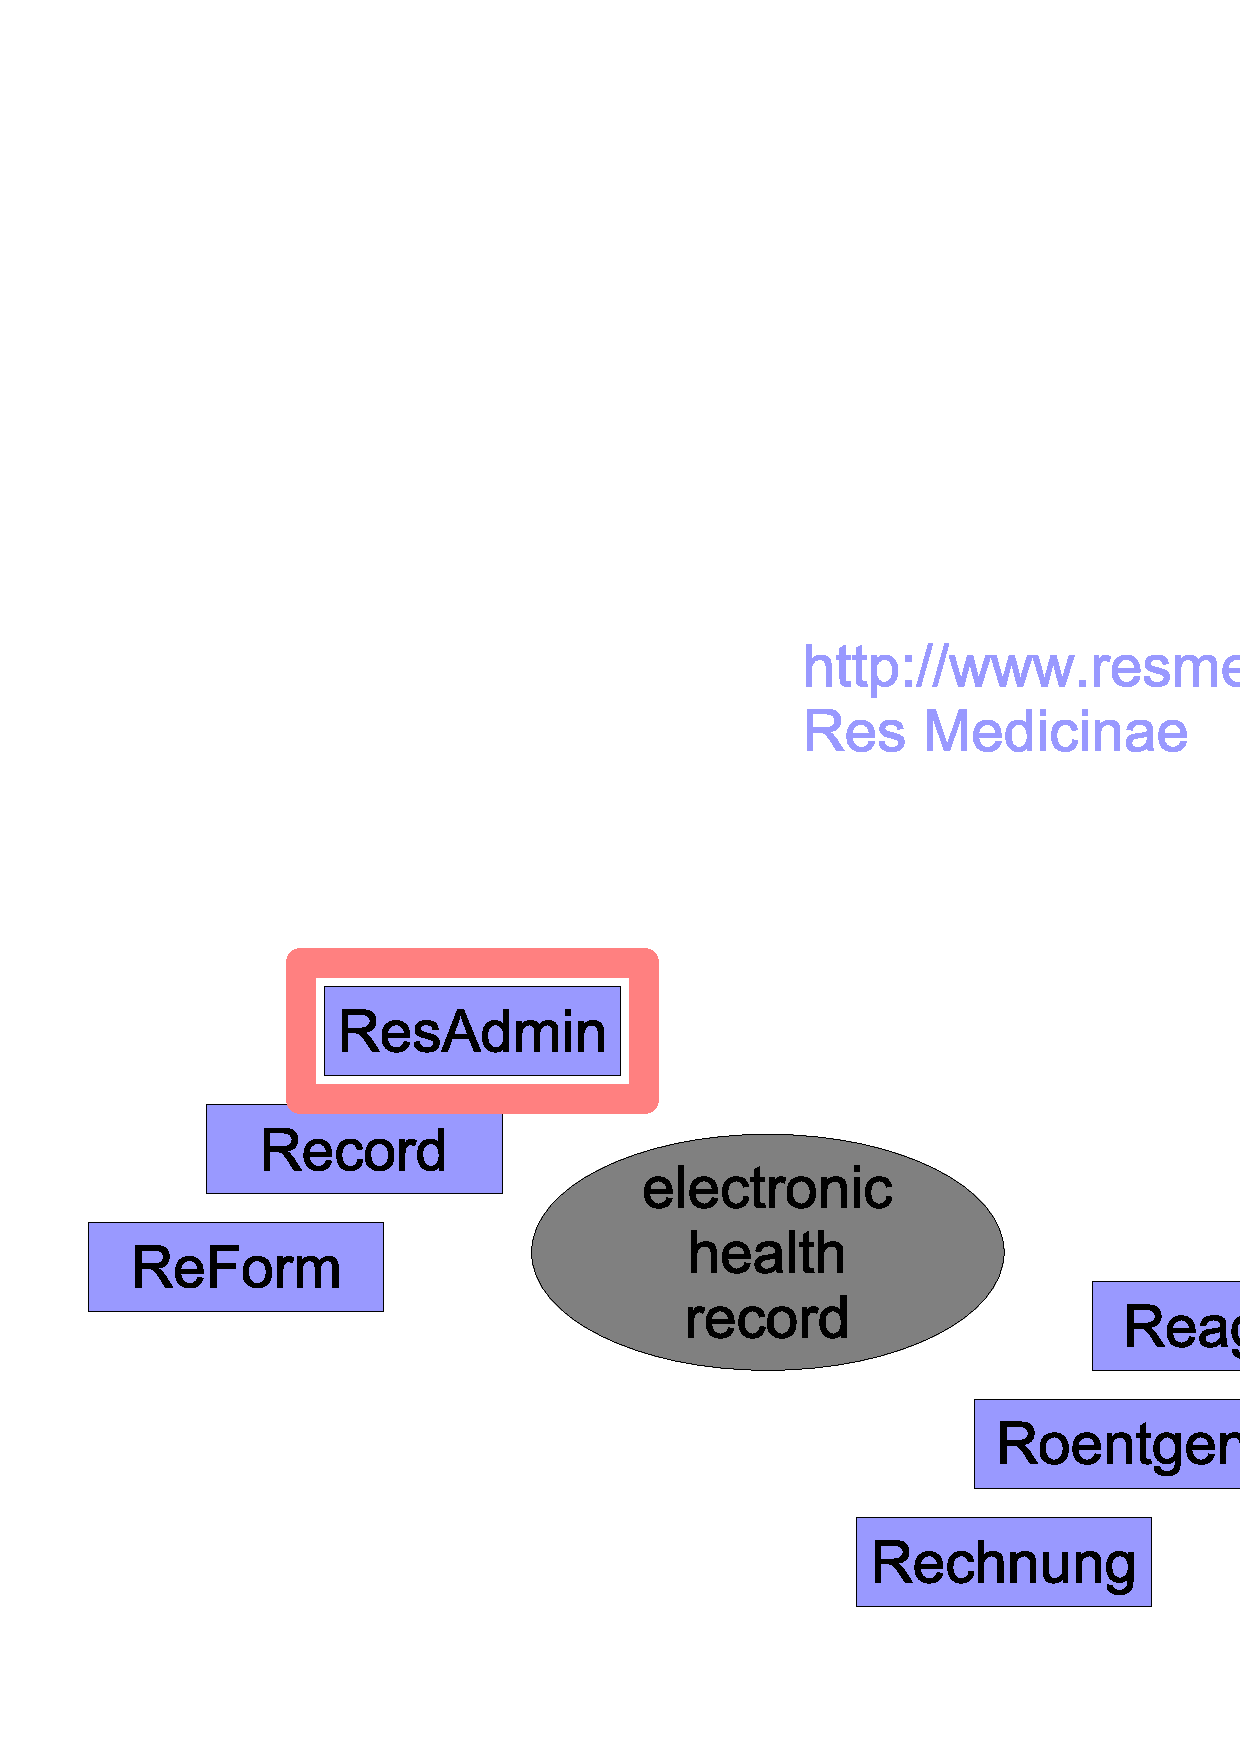
\includegraphics[scale=0.3,angle=-90]{graphic/core.pdf}
        \caption{Applications Grouped around an Electronic Health Record Core}
        \label{core_figure}
    \end{center}
\end{figure}

Figure \ref{core_figure} shows some of these modules, together with an EHR as
their central data structure.

